	%------------------第一章---------------------------
	\newpage
	\section{绪论}
    \subsection{超声波接近传感器的研究背景与意义}
    \subsubsection{超声波接近传感器的研究背景}
    超声波接近传感器是一种常用的非接触式测距传感器,广泛应用于工业自动化、机器人、无人驾驶等领域。随着技术的发展,超声波接近传感器的性能不断得到提高。\par    
    超声波接近传感器的发展经历了三个阶段。第一代超声波接近传感器采用固定式超声波传感器,能够实现对物体距离的测量,但是存在精度不高、抗干扰能力弱等问题。第二代超声波接近传感器采用微机处理技术和数字滤波技术,在一定程度上提高了抗干扰能力。第三代采用了新型材料和新技术,如MEMS技术、FPGA技术等,进一步提高了系统的测量精度、稳定性。
%    \subsubsection{超声波接近传感器国内外研究现状}
%    \paragraph{国内研究现状}
%	国内科研人员在超声波接近传感器上取得了突破性进展,主要集中在回波检测、超声换能器设计、发射脉冲选取等方面。
%	
%	在超声波换能器设计方面,2004年,通过对Vmos场效应管开关元件发射电路进行分析,矿业研究所的马庆云等研究发现,触发脉冲对超声波换能器的发射功率产生影响,最大发射功率对应的触发脉冲宽度是其谐振周期的$\frac{1}{2}$\upcite{超声波测距传感器的研究6}。这一发现对新型超声波换能器发射电路的研究具有指导作用,因为它可以克服传统调频超声波系统必须使用宽带超声传感器的问题,通过调整触发脉冲宽度来控制发射功率,从而实现对超声波发射信号的精确控制。
%	
%	2005年,李希胜等人在北京科技大学进行了一项研究,即窄带调频超声波距离检测。该技术不仅能够以极低的瞬时超声波功率实现极高的平均发射功率,而且还可以通过普通的超声波传感器实现,大大降低了传感器的成本。
%	
%	2006年,潘仲明对大检测范围超声波接近传感器进行了研究。该研究在谐振频率为23.5$kHz$基础上,研发出一种新型超声波接近传感器,其作用距离可以达到$31m$以上,测量误差低于$3\%$\upcite{超声波测距传感器的研究7}。
%		
%	在发射脉冲选取方面,程晓畅在2006年提出了一种基于雷达信号处理中的脉冲压缩技术的超声波发射脉冲选取方法,使用伪随机二进制序列来提供超声波发射的压缩信号,获得更高的信号功率和更小的脉冲宽度,从而提高了超声波信号的分辨率和检测精度\upcite{超声波测距传感器的研究8}。这种方法有效地解决了传统超声波检测中信号功率不足、信号宽度大等问题,为超声波检测技术的提高提供了重要的理论基础和实验支持。
%	
%	2008年,在嵌入式领域,杜晓同时考虑到测距量程和精度,利用$40kHz$与$20kHz$两种频率的超声波进行测距,将脉冲压缩技术很好的与双频超声测距技术相融合,使超声波接近传感器即可以增加检测范围,又能提高检测分辨率\upcite{超声波测距传感器的研究9}。
%		
%	2007年,陈平等人通过改良测距算法,设计了一种液位检测传感器。该超声波传感器考虑了温度对声速的影响,通过检测温度来对声速进行调整补偿,从而提高了检测分辨率。
%	
%	在机器人视觉领域,田志宏在2007年设计了一种可智能避障的自动轮椅车,并在传感器技术学报上发表了相关成果\upcite{超声波测距传感器的研究10}。王洪青研究出了一种并行超声波测距系统,该系统在各个方向安装传感器,实现了多传感器数据融合、实时检测距离的效果。
%	
%    \paragraph{国外研究现状}
%	同样,超声波接近传感器在国外也有了很大的发展。
%	
%	2013年2月,在伦敦帝国大学,Joseph Jackson,Rahul Summa等采用渡越时间法来进行超声波测距,该方法被应用于机器人、物体结构探测领域的研究\upcite{超声波测距传感器的研究11}。
%	
%	2010年12月,里斯本大学的研究人员Ricard Queiros和Francisc Corre Alegria提出了一种新型的超声波接近传感器测距方法。该方法利用了交叉相关联和正弦发生器技术,提高了传感器的精度。交叉相关技术通过将发送信号与接收信号相融合,检测超声波在空气中传播的时间,从而精确测量距离;正弦发生器则可以检测超声波传播过程中的相移,进而提高测距的分辨率。
%	
%	2011年,JiDe Huang和Chih Kung Lee在康奈尔大学提出了一种新的高精度超声波测距系统,该系统采用基于峰值检测和干涉技术的方法。该超声波测距系统的特点是通过硬件设计提高了测距系统的精度,而不依赖于复杂的算法,不仅提高了传感器的精度,还没有使得成本增加。\upcite{超声波测距传感器的研究14}。
%	
%    
    \subsubsection{超声波接近传感器的研究意义}
    TUSS4470芯片作为一种新型的超声波传感器芯片,具有高精度、低功耗和多种工作模式等特点,可以满足现代工业和自动化控制对于测量、检测、控制和导航等方面的需求。因此,基于TUSS4470芯片的超声波接近传感器的研究成为了一个热门话题,其可以应用于智能家居、无人机、自动驾驶车辆、机器人等领域,具有广阔的应用前景和市场前景。\par
    此外,在传统的超声波驱动控制电路中,一般是采用模拟电路或者单片机来控制。由模拟电路驱动的超声波传感器抗干扰性差,而由单片机驱动的超声波传感器,由于其使用外部中断触发的机制,导致无法精确控制时序逻辑,从而难以达到与超声探头匹配的驱动频率,而超声波传感器的检测精度直接取决于其发出脉冲宽度的精度\upcite{CPLD在超声波传感器驱动控制电路中},当脉冲宽度无法匹配时将使得传感器的精度降低,因此使用CPLD芯片控制产生精确的脉冲宽度对提高传感器的检测精度有着十分重要的意义。\par
    本设计采用型号为EPM240T100C5N的MAX II系列芯片,它是一种高集成度、电可擦除、CMOS宏阵列可编程逻辑器件\upcite{基于STM32和超声波测距的倒车雷达预警系统设计},可以产生ns级别的控制信号\upcite{CPLD芯片介绍},配合TUSS4470超声驱动芯片,可精确控制发送脉冲的次数、频率以及脉冲宽度。同时,CPLD芯片编程采用时序逻辑,可精准控制各引脚输出波形的时序,这让超声检测策略可以变得更加丰富合理。
    \subsection{超声波接近传感器的原理}
    \subsubsection{超声波介绍}
      超声波作为机械波,可以在各种介质中传播。人类可识别20Hz-20kHz频率的声音,高于该范围的为超声波,低于为低频声波。超声波抗干扰性强,不易受外界干扰而波动,且超声波反射过程中,射出角和射入角相等,适用于距离检测\upcite{车载可视倒车雷达预警系统的研制}。
      
      超声波的波动方程如式\ref{波动方程}所示。
    \begin{equation}
    	U=U(x)cos(\omega t+kx)
    	\label{波动方程}
    \end{equation}
	式中\quad$x$---传播距离;\par
	\quad$\omega$---频率
	\begin{equation}
		U(x)=U_0 e^{-\alpha x}
		\label{振幅方程}
	\end{equation}
	式中\quad$U(x)$---振幅;\par
		\quad$\alpha$---衰减系数
	\begin{equation}
		\alpha=a f^2
		\label{衰减指数}
	\end{equation}
	式中\quad $a$---介质常数;\par
	   \quad $f$---振动频率\par
    根据式\ref{衰减指数}我们可以得出,当频率变高时,衰减系数增大,传播距离变短。但考虑到声波的指向性,超声波频率应当是越高越好。综合考虑,我们选取$f$=300kHz的换能器。
    \subsubsection{超声换能器的原理与结构}
    超声换能器是一种能量转换装置,可将其他能与超声能相互转换。超声换能器包括电声型和流体动力型\upcite{面向机器人安全避障的MEMS压电超声接近觉传感器的研究39}。
    电声型超声换能器主要包括压电换能器、磁质伸缩换能器和静电换能器三种\upcite{车载可视倒车雷达预警系统的研制}。
    流体动力型超声换能器主要包括气体和液体两种类型。其中,气体型是利用气体流动产生的声波进行能量转换,液体型则是利用液体流动产生的声波进行能量转换。这两种传感器在实际应用中具有一定的局限性,主要是在响应频率、灵敏度、稳定性等方面存在一定的问题\upcite{车载可视倒车雷达预警系统的研制13}。\par
    电声型换能器中最常用的为压电超声换能器,它将电能与振动相互转换,从而实现检测。压电换能器中一般使用双压电晶片,分别完成发射接收工作。当晶片受到电信号激励时,会产生振动,从而带动周围介质产生超声波;而当晶片收到声波时,会发生微量变形,从而产生可供检测的电信号\upcite{车载可视倒车雷达预警系统的研制15}。
    \begin{figure}[!h]

    	\begin{minipage}{0.5\textwidth}
    		\centering
    		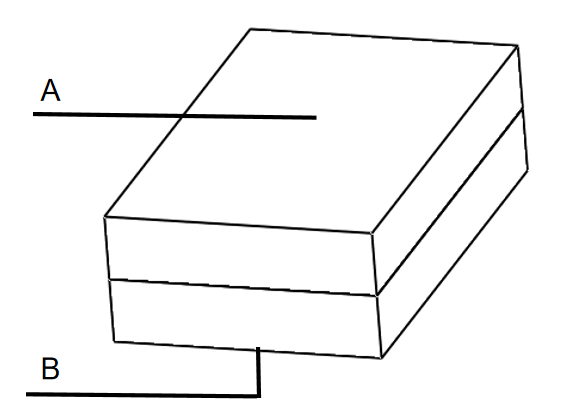
\includegraphics[height=4cm]{figure/双压电晶片示意图.png}
    		\caption{双压电晶片示意图\upcite{51单片机超声波测距仪防撞报警倒车雷达设计}}
    		\label{双压电晶片示意图}
    	\end{minipage}
    \begin{minipage}{0.5\textwidth}
    	\centering
    	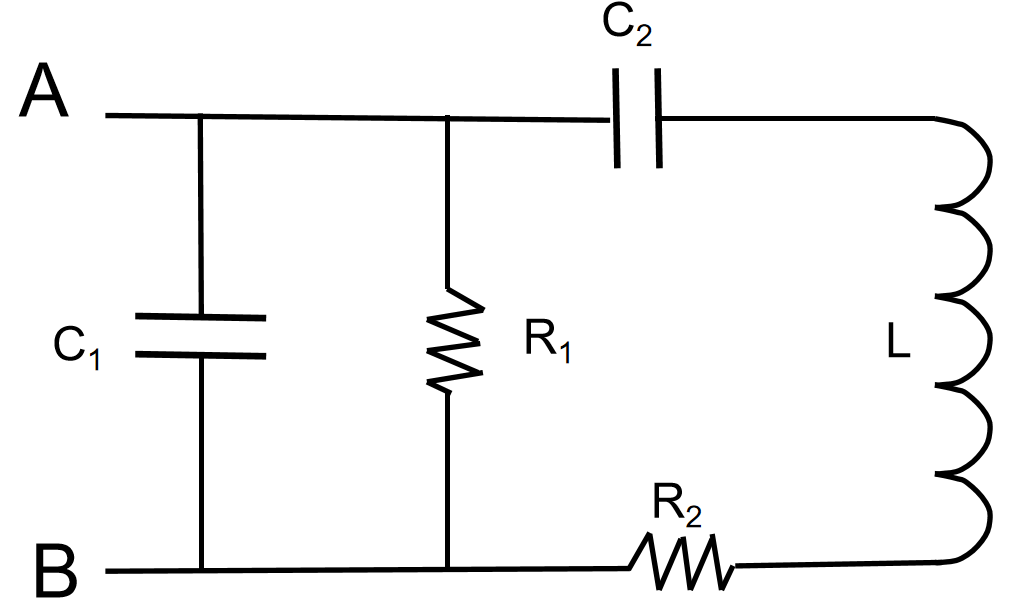
\includegraphics[height=4.25cm]{figure/双压电晶片等效电路.png}
    	\caption{双压电晶片等效电路图\upcite{51单片机超声波测距仪防撞报警倒车雷达设计}}
    	\label{双压电晶片等效电路图}.
    \end{minipage}
    \end{figure}

    双压电晶片如图\ref{双压电晶片示意图},对两晶片施加交流电压,如果电场方向与极化方向相同,则起到了增强极化作用的效果,反之则抑制了该效果,利用这种现象,晶片可产生一定频率的交变形变,当这种形变传递到介质中时,就形成了超声波。双压电晶片的等效电路如图\ref{双压电晶片等效电路图}所示\upcite{51单片机超声波测距仪防撞报警倒车雷达设计}。\par

    压电陶瓷晶片有一个固定的谐振频率,即中心频率$f$。脉冲信号频率与施加交变电场频率越相近,传感器的精度就越高。当所用材料不变时,改变晶片尺寸,就可改变其中心频率,从而可以得到具有各种中心频率的超声换能器\upcite{车载可视倒车雷达预警系统的研制16}。
    如图\ref{超声换能器结构图}所示,为超声换能器的一般组成。
    \begin{figure}[!h]
    	\centering
    	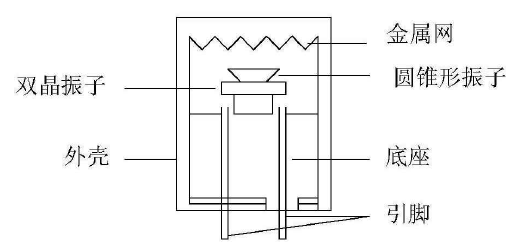
\includegraphics[width=7cm]{figure/超声换能器结构图.png}
    	\caption{超声换能器结构图\upcite{车载可视倒车雷达预警系统的研制16}}
    	\label{超声换能器结构图}
    \end{figure}
\newpage
    \subsubsection{超声波接近传感器的检测原理}
    \paragraph{连续波相位检测法(CW法))}
    连续波相位检测法的原理如图\ref{连续波相位检测法}。对比发射与回波信号间存在的相位差异,可获得时间延迟,从而计算出与物体的距离\upcite{面向机器人安全避障的MEMS压电超声接近觉传感器的研究34}。\par
    \begin{figure}[!h]
    	\centering
    	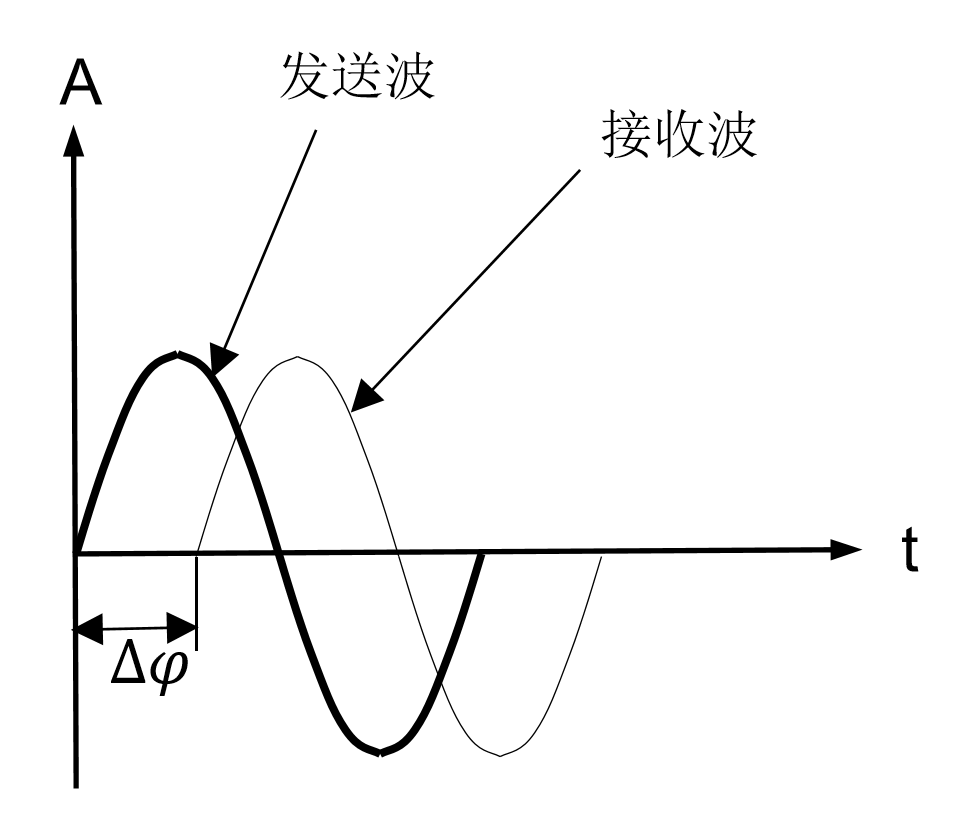
\includegraphics[width=6cm]{figure/连续波相位检测法.png}
    	\caption{连续波相位检测法\upcite{面向机器人安全避障的MEMS压电超声接近觉传感器的研究34}}
    	\label{连续波相位检测法}
    \end{figure}\par


    假设 发射 的 声 波信 号 为 :
    \begin{equation} 
    	u_1=U(x)sin(\omega t + \varphi)
    \end{equation}
式中\quad$\varphi$---初始相位角\par

则回波信号为:
\begin{equation}
	u_2=U(x)sin(\omega t + \varphi + \omega \cdot{\Delta \varphi})
\end{equation}
式中\quad$b$---声速\par
\quad$\Delta \varphi$---相位差\par
发射接收信号的相位差为:
\begin{equation}
	\Delta \varphi=\frac{2D}{b}
\end{equation}
式中\quad$D$---与检测物体的距离\par
联立上述公式,可得到与物体间的距离为\upcite{面向机器人安全避障的MEMS压电超声接近觉传感器的研究35}:
\begin{equation}
	D=\frac{b}{2\omega}\cdot \Delta \varphi=\frac{b}{4\pi f}\cdot(2\pi n + \varphi_i)
\end{equation}
式中\quad$n$---整周期的个数;\par
\quad$\varphi_i$---不完整周期的相位值\par
   
    \paragraph{飞行时间法}
    飞行时间法\upcite{面向机器人安全避障的MEMS压电超声接近觉传感器的研究35}如图\ref{飞行时间检测法}。脉冲发射接收存在时间差,这个时间差即为飞行时间$t_2$:
    \begin{equation}
    	t_2=\frac{l}{b}
    \end{equation}
式中\quad$l$---声波传播距离;\par
\quad$b$---声速\par

    \begin{figure}[!h]
    	\centering
    	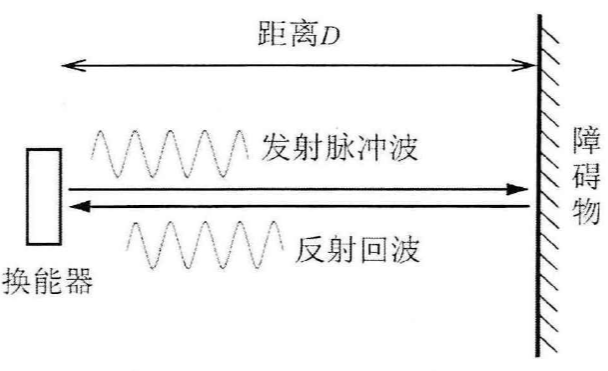
\includegraphics[width=6cm]{figure/飞行时间检测法.png}
    	\caption{飞行时间检测法\upcite{面向机器人安全避障的MEMS压电超声接近觉传感器的研究35}}
    	\label{飞行时间检测法}
    \end{figure}\par
    距离$D$的计算公式为:
    \begin{equation}
    	D=\frac{l}{2}=\frac{bt_2}{2}
    \end{equation}\par
	在该方法中,如何精确的获取$t_2$尤其重要,直接关系到传感器的测距精度。
	常见获取飞行时间的方法有:互相关函数法、固定阈值法和包络峰值法。其中较常使用的是固定阈值法,即设计一个阈值,当回波信号幅值超过该阈值时,视为接收到了回波,以此来换算飞行时间。\par
	       
\subsection{本设计的主要研究内容和论文结构安排}
\subsubsection{主要研究内容}
本设计针对生产线上检测钢化玻璃到位问题,设计了一种稳定性好、灵活性高、应用场景丰富的超声波接近传感器。
本设计的主要研究内容包括了超声波接近传感器的硬件设计、软件设计和实验设计。\par
硬件设计包括了原理图设计和PCB设计,软件设计包括了TUSS4470集成芯片配置、脉冲信号产生、物体检测三个部分的程序设计,以及波形仿真。实验设计部分包括了设计实验进行性能参数测试、稳定性测试和回波特性测试。

\subsubsection{论文结构安排}
本文各章节的主要内容如下:

第二章:提出了超声波接近传感器的总体设计,初步介绍各个部分的设计流程与方法步骤。然后讲解了在本设计所涉及到的检测原理。

第三章:介绍了硬件电路方面的工作,讲解了原理图设计和PCB设计的流程。原理图部分的设计分为三部分,分别为:超声波接近传感器控制电路设计、TUSS4470芯片外围电路设计、检测计数电路设计。PCB设计部分主要介绍了TUSS4470外围电路PCB设计,讲解了在PCB设计过程中遵循的几大原则,用于减小各类信号相互之间的干扰,包括了电容、二极管等器件摆放位置优先级,分离接地,铺铜规则等。

第四章:介绍了软件设计部分的工作,首先讲解了传感器所采取的检测策略,然后进行程序的总体设计,根据功能将程序分为了四个模块,分别为:控制模块、SPI模块、脉冲产生模块和检测计数模块。之后分别详细讲解了各个模块的功能、实现原理以及程序流程图。在完成了程序设计方面的工作后,又介绍了波形的仿真模拟过程,并对结果进行了分析。

第五章:设计实验测试传感器的性能以及检测策略的可行性。首先讲解了实物的焊接与调试流程,给出了调试过程中所测得的各引脚波形,然后介绍了实验所用的实验器材,包括虚拟示波器、直尺、各种板材等。最后进行实验,测试了传感器的性能参数、检测策略可行性以及回波特性,给出了实验的结果以及后续分析。

第六章:总结传感器的缺点,提出改进方案,并且对未来进行展望。

    \subsection{本章小结}
    本章主要介绍了超声波接近传感器的研究背景和意义,在研究背景中介绍了超声波接近传感器总体的发展,然后引出本设计的研究意义是为了设计精度高、稳定性好的传感器。在第二节主要介绍了传感器主要涉及到的原理,包括超声波振幅衰减原理、超声换能器发射脉冲与检测回波信号的原理。在本章的最后一节,则是介绍了本设计的主要研究内容和论文结构安排,并且简单介绍了后几章所包含的内容。